

\label{sec:resultados}

%-XXXXXXXXXXXXXXXXXXXXXXXXXXXXXXXXXXXXXXXXXXXXXXXXXXXXXXXXXXXX
% Este párrafo tiene información repetida. Se debe
% decir al iniciar esta sección que por cada etpata de la 
% Metdología se presentarán los resultados para dar cumplimiento a
%los objetivos y ahí pueden referenciar la tabla de la metodología
% que conecta cada etapa de la metodología y objetivos.
%-XXXXXXXXXXXXXXXXXXXXXXXXXXXXXXXXXXXXXXXXXXXXXXXXXXXXXXXXXXXX
%-XXXXXXXXXXXXXXXXXXXXXXXXXXXXXXXXXXXXXXXXXXXXXXXXXXXXXXXXXXXX
% Deben revisar el tema de las siglas, pues hay muchas repeticiones
% de explkicación de siglas y otras faltan por definición.
%-XXXXXXXXXXXXXXXXXXXXXXXXXXXXXXXXXXXXXXXXXXXXXXXXXXXXXXXXXXXX

% En esta sección se presentan los resultados preliminares del proceso de modelamiento para la estimación del Índice de Pobreza Multidimensional (IPM) 2024 mediante un enfoque de estimación para áreas pequeñas. El ejercicio desarrollado tuvo como propósito construir y evaluar una primera aproximación metodológica que permitiera combinar la estimación directa del IPM a nivel departamental, proveniente de la Encuesta Nacional de Calidad de Vida (ECV) 2024, con un conjunto de covariables auxiliares disponibles a nivel municipal.





%-XXXXXXXXXXXXXXXXXXXXXXXXXXXXXXXXXXXXXXXXXXXXXXXXXXXXXXXXXXXX
% Este párrafo corresponde a metodología
% Es mejor hablar de estimación del IPM en lugar de predición del IPM
%-XXXXXXXXXXXXXXXXXXXXXXXXXXXXXXXXXXXXXXXXXXXXXXXXXXXXXXXXXXXX

% El proceso analítico se estructuró en cuatro momentos principales:
% \begin{enumerate}
%     \item Se construyó una base analítica departamental a partir de la agregación de covariables municipales.
%     \item Se ajustaron distintos modelos lineales exploratorios con diferentes combinaciones de variables.
%     \item Se estimaron dos variantes del modelo Fay–Herriot.
%     \item Se aplicaron los coeficientes obtenidos para generar una predicción sintética municipal del IPM 2024, acompañada de ejercicios preliminares de validación y diagnóstico espacial.
% \end{enumerate}


%-XXXXXXXXXXXXXXXXXXXXXXXXXXXXXXXXXXXXXXXXXXXXXXXXXXXXXXXXXXXX
% Se deben crear secciones o etapas con el mismo nombre de la
% metodología para que no se bpierdan los jurados.
%-XXXXXXXXXXXXXXXXXXXXXXXXXXXXXXXXXXXXXXXXXXXXXXXXXXXXXXXXXXXX



%--------------------------------------------------------------------------------------
\section{Limpieza, filtrado y reglas explícitas}

La normalización a escala 0-1 de las variables de proporción y cobertura, descrita en la Sección~\ref{sec:metodologia}, se verificó sobre la fuente única de covariables. La depuración permitió consolidar una base municipal 2024 con códigos municipales únicos y variables cuantitativas en formatos homogéneos. Las variables de cobertura y proporción quedaron expresadas en escala 0–1. Los controles de consistencia permitieron identificar una advertencia en las variables de recaudo, sin incidencia sobre los escenarios finalmente modelados.

La verificación de alineación por llave municipal identificó una advertencia en las variables de recaudo: la coherencia entre el recaudo total del impuesto de industria y comercio y su valor per cápita arrojó una correlación de 0.5322, por debajo del umbral esperado bajo un cruce correcto. Esta advertencia no tuvo incidencia sobre las especificaciones finalmente modeladas, dado que estas variables no integraron ninguno de los tres escenarios finalmente evaluados, la inconsistencia identificada no afectó la estimación de M1, M2 o M3. La verificación de plausibilidad de los municipios más poblados (Bogotá D.C., Medellín y Santiago de Cali) no arrojó anomalías. La base departamental quedó conformada, como se esperaba, por 33 dominios.

%--------------------------------------------------------------------------------------
\section{Construcción de la variable respuesta}

La estimación directa del IPM 2024 presentó valores entre 5.4 en Bogotá D.C. Y 70.2 en Vichada, con una media de 17.68 para los 33 dominios considerados. La varianza de muestreo asociada a estas estimaciones osciló entre 0.49 y 5.29, evidenciando diferencias en el nivel de precisión de las estimaciones directas entre departamentos.

Esta heterogeneidad en la varianza de muestreo resulta relevante para las formulaciones evaluadas, dado que la incertidumbre asociada a cada estimación departamental se incorpora explícitamente durante el proceso de ajuste. De esta manera, los departamentos no aportan información con el mismo nivel de precisión a la calibración de los modelos. 

Las 33 estimaciones directas departamentales constituyeron la variable observada de referencia para la calibración de las tres formulaciones. Asimismo, durante la validación por exclusión de dominio (\textit{Leave-One-Domain-Out}, LODO), la estimación directa correspondiente al departamento excluido se utilizó exclusivamente como valor observado de referencia para evaluar la predicción generada sin la participación de dicho dominio en el ajuste. Esta separación permitió evaluar posteriormente la capacidad predictiva fuera de dominio mediante las métricas definidas en la metodología.
%--------------------------------------------------------------------------------------
\section{Construcción de variables predictoras y escenarios covariables}

La agregación departamental ponderada, descrita en la Sección~\ref{sec:metodologia}, se aplicó sobre la muestra analítica común a las tres formulaciones, generando los 33 promedios departamentales empleados en la calibración. El número de municipios agregados por departamento fue marcadamente heterogéneo, entre 1 y 125, lo que confirma la pertinencia del esquema de ponderación. Un promedio aritmético simple asignaría la misma contribución a municipios con poblaciones de referencia sustancialmente diferentes, mientras que el promedio ponderado preserva la importancia relativa de cada unidad de acuerdo con la población expuesta al indicador correspondiente.

Los promedios departamentales resultantes conservaron variación sustantiva entre dominios en las siete covariables del escenario Completo, como se muestra en la Tabla~\ref{tab:rangos-covariables-depto}.

\begin{table}[!htbp]
\centering
\small
\caption{Rango de las covariables agregadas a escala departamental, escenario Completo (33 dominios).}
\label{tab:rangos-covariables-depto}
\renewcommand{\arraystretch}{1.25}
\begin{tabular}{l c c}
\hline
\textbf{Covariable} & \textbf{Mínimo} & \textbf{Máximo} \\
\hline
Repitencia escolar (\%)                     & 6.66  & 18.50 \\
Tasa de matriculación 5-16 años (\%)        & 53.79 & 100.00 \\
Índice de infraestructura básica (\%)       & 20.79 & 100.00 \\
Cobertura de energía rural (\%)             & 21.89 & 100.00 \\
Mortalidad infantil (por mil nacidos vivos) & 6.70  & 30.39 \\
Aseguramiento en salud capado (\%)          & 59.42 & 100.00 \\
Luminosidad nocturna (log)                  & 0.22  & 2.78 \\
\hline
\end{tabular}
\end{table}

%--------------------------------------------------------------------------------------
\section{Identificación de datos faltantes, ventanas temporales y estrategia de validación}

La aplicación del criterio común de completitud, descrito en la Sección~\ref{sec:metodologia}, condujo a una muestra analítica de 1{,}121 municipios de los 1{,}122 que conforman el universo municipal del país, con un único municipio excluido por información incompleta en alguna de las covariables del escenario Completo o en los denominadores poblacionales de ponderación. Esta misma muestra fue empleada de manera común por las tres formulaciones.

Tanto la variable respuesta como las covariables auxiliares correspondieron exclusivamente al año 2024, sin combinar información de otros periodos en la calibración de los modelos. La validación por exclusión de dominio (LODO) se aplicó de manera independiente a las tres formulaciones bajo los tres escenarios de covariables, cuyos resultados se presentan en las Secciones~\ref{sec:res-fh} en adelante.

%--------------------------------------------------------------------------------------
\section{Análisis exploratorio y diagnóstico espacial}
\label{sec:analisis-exploratorio}

Las asociaciones bivariadas entre la estimación directa del IPM y las covariables agregadas a escala departamental mostraron, en general, direcciones consistentes con su interpretación conceptual. La repitencia escolar se asoció positivamente con el IPM directo, mientras que la infraestructura básica y el aseguramiento en salud mostraron asociaciones negativas.

Como diagnóstico espacial previo a la incorporación de un componente CAR, se evaluó el índice global de Moran sobre los residuos obtenidos bajo los tres escenarios exploratorios. Para examinar la sensibilidad del resultado a la definición de vecindad, se utilizaron matrices construidas mediante $k$ vecinos más cercanos, con $k=3$, $k=4$ y $k=5$. Los resultados se presentan en la Tabla~\ref{tab:moran-exploratorio}.

El escenario Completo no presentó evidencia estadísticamente significativa de autocorrelación espacial residual bajo ninguno de los tres esquemas evaluados. Este resultado es compatible con una menor estructura espacial remanente después de considerar el conjunto de covariables incluido en esta especificación, aunque no permite atribuir dicha ausencia exclusivamente a las variables incorporadas.

En contraste, el escenario Parsimonioso presentó autocorrelación espacial positiva y estadísticamente significativa para $k=4$ ($I=0.191$, $p=0.019$) y $k=5$ ($I=0.150$, $p=0.035$). El escenario Alternativo de vivienda presentó evidencia significativa únicamente para $k=4$ ($I=0.178$, $p=0.022$); para $k=3$ y $k=5$ los resultados no alcanzaron significancia estadística al 5\,\%.

En conjunto, estos resultados muestran que la presencia de dependencia espacial residual varía según la especificación de covariables y la estructura de vecindad considerada. La evidencia observada, particularmente en los escenarios Parsimonioso y Alternativo de vivienda, sustentó la evaluación posterior de una formulación que incorporara explícitamente un componente espacial municipal mediante una estructura CAR de rango reducido.

Este diagnóstico corresponde a una etapa exploratoria previa a la estimación de M3 y debe distinguirse del índice de Moran calculado posteriormente sobre el efecto espacial estimado del modelo CAR, el cual caracteriza la estructura del componente espacial incorporado y no constituye una medida de autocorrelación residual.

\begin{table}[!htbp]
\centering
\small
\caption{Estadístico de Moran sobre los residuos de los escenarios exploratorios, bajo distintos esquemas de vecindad por $k$-vecinos más cercanos.}
\label{tab:moran-exploratorio}
\renewcommand{\arraystretch}{1.25}
\begin{tabular}{c l c c}
\hline
\textbf{Vecinos ($k$)} & \textbf{Escenario} & \textbf{Moran I} & \textbf{Valor p} \\
\hline
3 & Completo             & $-0.042$ & 0.514 \\
3 & Parsimonioso         & $0.146$  & 0.076 \\
3 & Alt. vivienda        & $0.141$  & 0.079 \\
4 & Completo             & $0.065$  & 0.151 \\
4 & Parsimonioso         & $0.191$  & 0.019 \\
4 & Alt. vivienda        & $0.178$  & 0.022 \\
5 & Completo             & $-0.008$ & 0.372 \\
5 & Parsimonioso         & $0.150$  & 0.035 \\
5 & Alt. vivienda        & $0.082$  & 0.109 \\
\hline
\end{tabular}
\end{table}

%--------------------------------------------------------------------------------------
\section{Preprocesamiento específico para la modelación}

La construcción de la matriz de adyacencia municipal bajo el criterio de contigüidad tipo Reina, descrita en la Sección~\ref{sec:metodologia}, identificó dos unidades sin vecinos dentro de la red espacial: San Andrés y Providencia, pertenecientes al Archipiélago de San Andrés, Providencia y Santa Catalina. Esta condición responde a su carácter insular, dado que ninguna de estas unidades comparte un límite terrestre con otro municipio bajo el criterio de contigüidad empleado.

La estructura de vecindad resultante presentó tres componentes conexos: un componente principal conformado por los municipios continentalmente conectados y dos componentes aislados correspondientes a San Andrés y Providencia. Las 1,121 unidades de la muestra analítica contaron con geometría disponible; sin embargo, las dos unidades insulares presentaron grado cero en la matriz de adyacencia. En consecuencia, la construcción de la base espacial de rango reducido se realizó sobre los municipios con al menos un vecino, mientras que las unidades aisladas conservaron su componente fijo de covariables, pero no recibieron contribución del efecto espacial CAR.

La reducción de rango del efecto espacial, aplicada para hacer viable su estimación a partir de los 33 dominios departamentales utilizados en la calibración, conservó los seis componentes asociados a los mayores autovalores de la matriz de vecindad normalizada. Los autovalores correspondientes a los patrones espaciales retenidos se ubicaron entre 0.9847 y 1, indicando que la representación reducida conserva los patrones de autocorrelación espacial positiva de mayor escala presentes en la red municipal.

%--------------------------------------------------------------------------------------
\section{Implementación de modelos exploratorios mediante mínimos cuadrados ordinarios}

El ajuste mediante mínimos cuadrados ordinarios (OLS) se utilizó como una etapa diagnóstica para caracterizar el comportamiento de los tres escenarios de covariables definidos previamente. Los resultados mostraron un ajuste global relativamente alto en los tres casos, aunque con diferencias en la complejidad de las especificaciones y en el nivel de colinealidad entre los predictores.

El escenario Completo presentó el mayor coeficiente de determinación ajustado ($R^2_{\text{aj}}=0.8643$), seguido del escenario Parsimonioso ($R^2_{\text{aj}}=0.8178$) y del escenario Alternativo de vivienda ($R^2_{\text{aj}}=0.7904$). Sin embargo, el escenario Completo incorporó siete covariables además del intercepto, lo que produjo una razón de 4.12 dominios por parámetro, inferior a la referencia de cinco observaciones por parámetro utilizada como criterio diagnóstico. En contraste, los escenarios Parsimonioso y Alternativo de vivienda, ambos conformados por cuatro covariables, alcanzaron una razón de 6.60 dominios por parámetro.

La Tabla~\ref{tab:ols-resultados} resume estas diferencias. El diagnóstico de colinealidad mostró que el escenario Completo presentó el mayor factor de inflación de varianza, con un VIF máximo de 5.005, ubicado en el límite utilizado como referencia para identificar posibles problemas de redundancia entre covariables. En los escenarios Parsimonioso y Alternativo de vivienda, los valores máximos fueron considerablemente menores, con 2.477 y 2.729, respectivamente, sin evidencia de colinealidad severa.

\begin{figure}[!htbp]
\centering
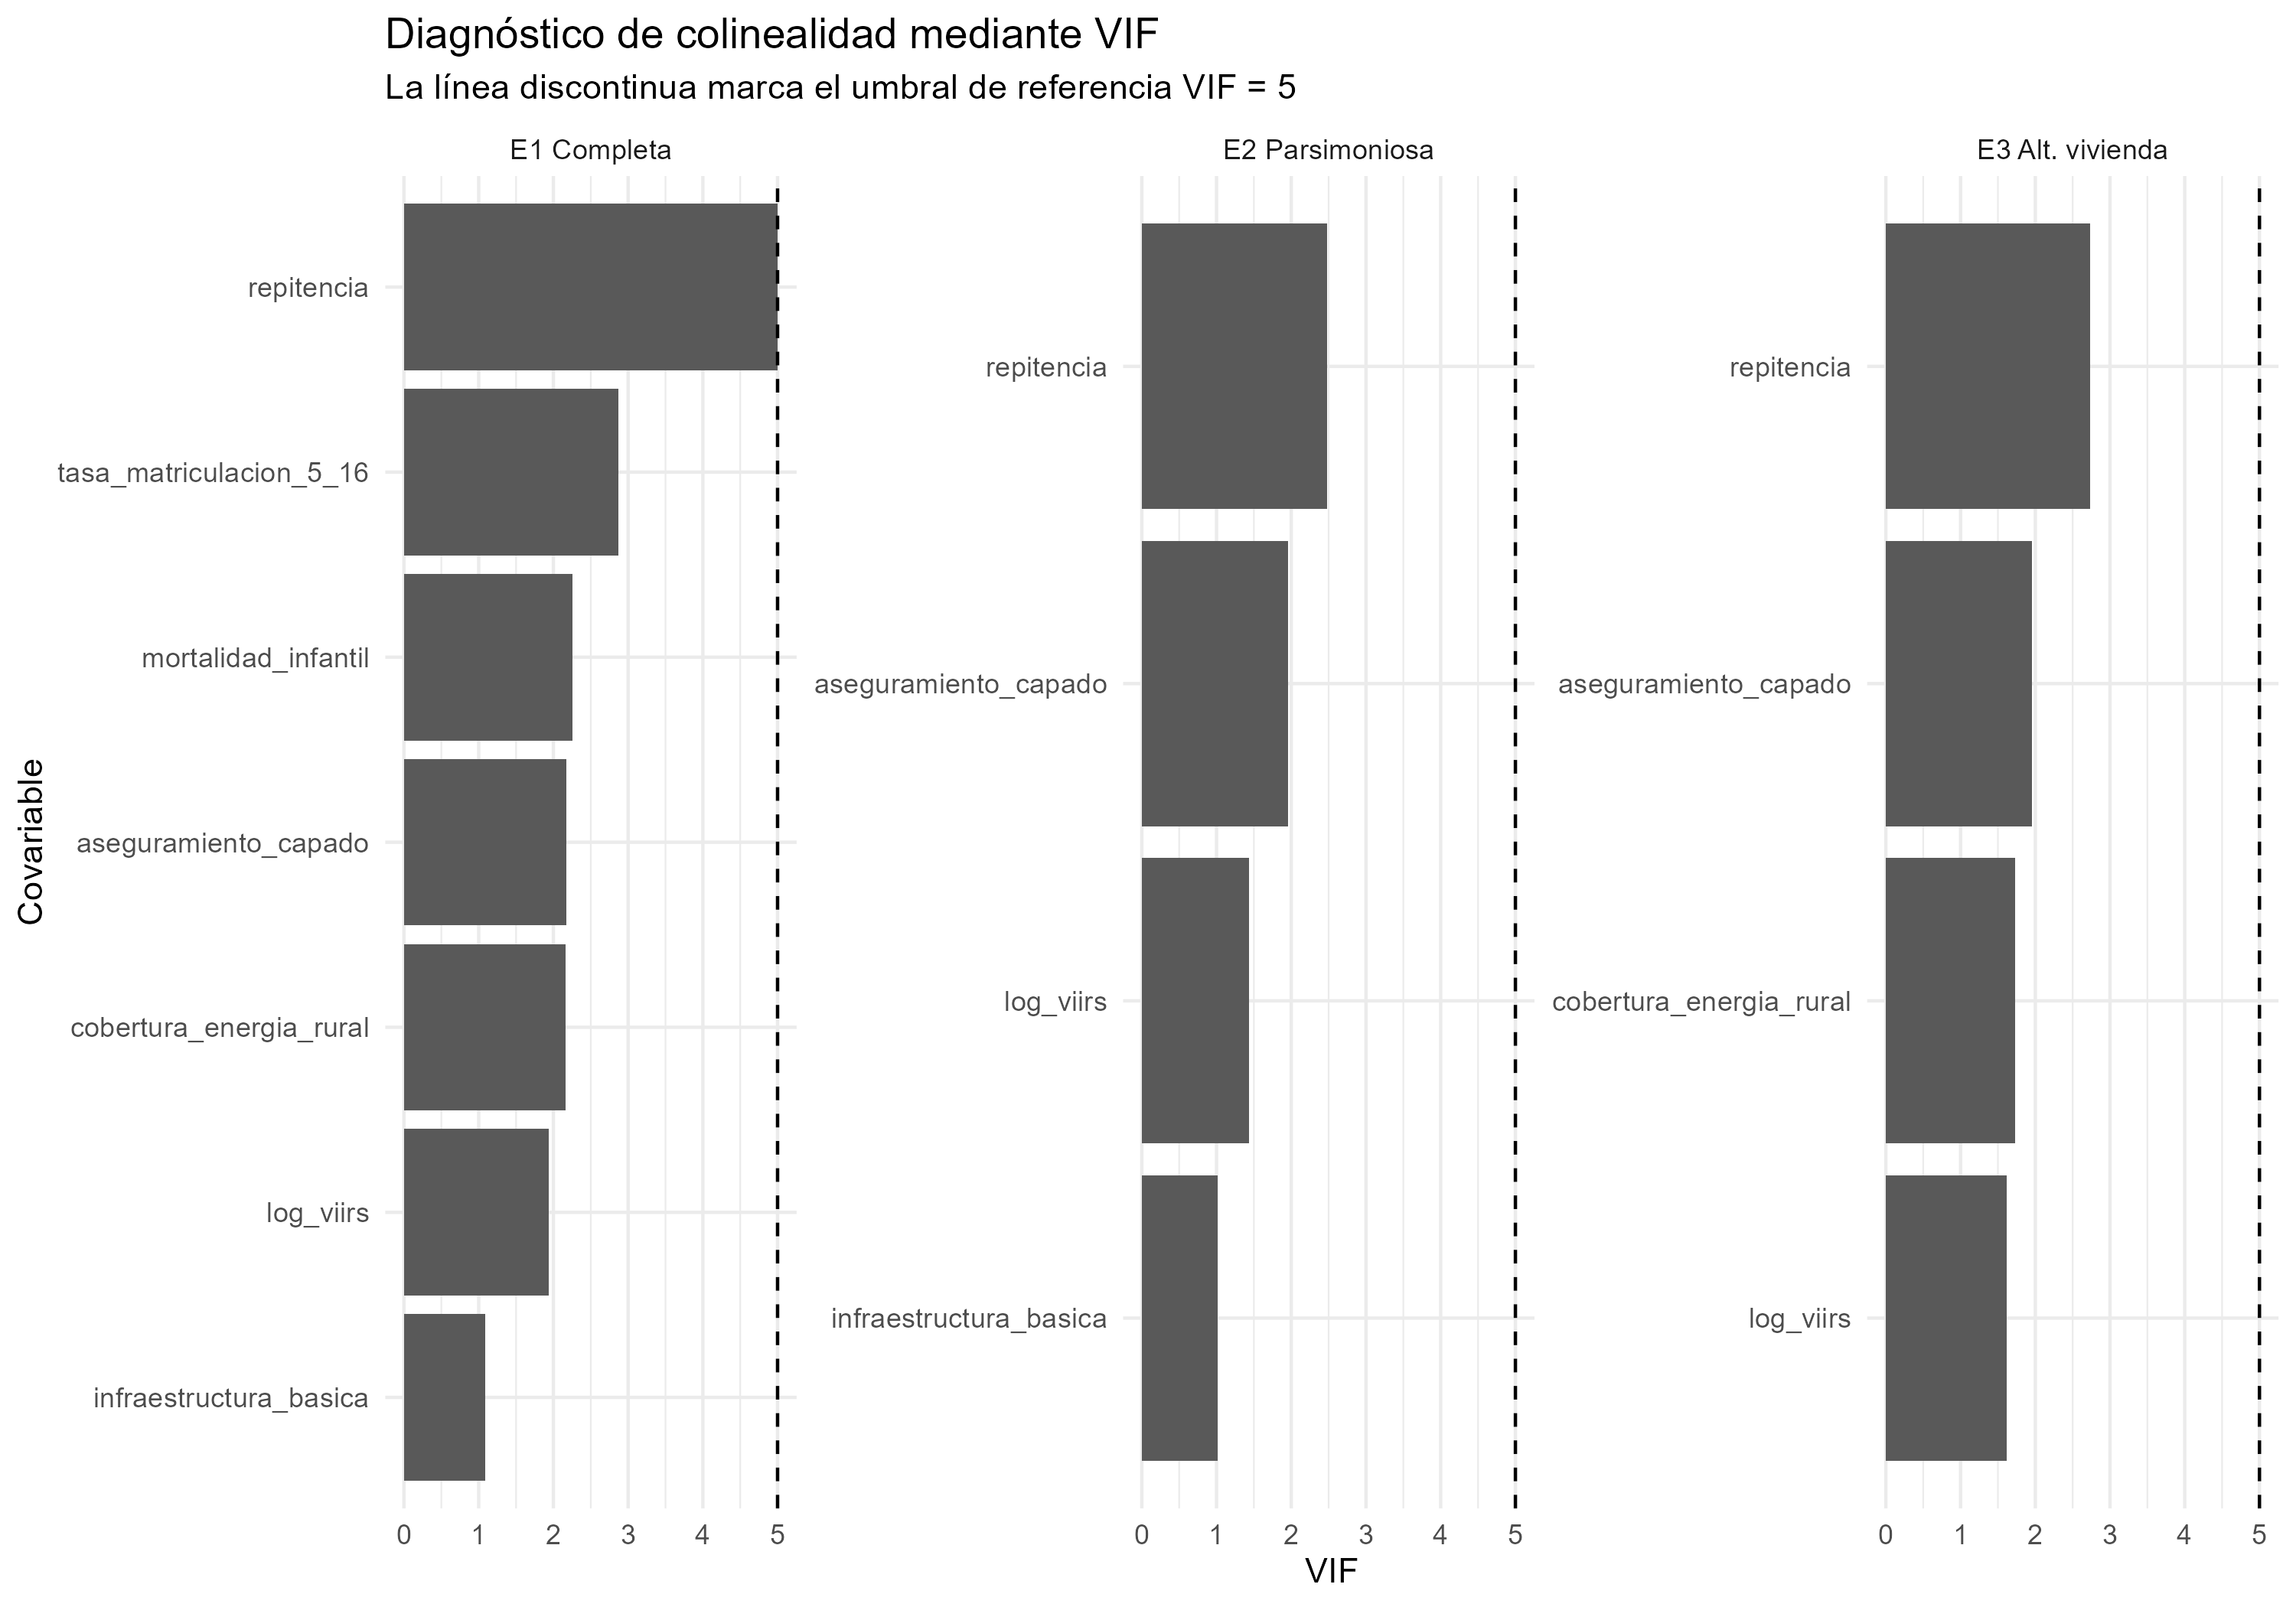
\includegraphics[width=0.95\textwidth]{fig/figures/diagnostico_VIF_escenarios.png}
\caption{Factores de inflación de la varianza por covariable y escenario.}
\label{fig:diag-VIF}
\end{figure}

La revisión de los coeficientes mostró, en términos generales, una dirección consistente con la interpretación conceptual de las covariables. La tasa de repitencia escolar presentó signo positivo en los tres escenarios, indicando una asociación directa con el IPM departamental. Por su parte, el índice de infraestructura básica, la cobertura de energía rural, el aseguramiento en salud capado y la luminosidad nocturna presentaron coeficientes negativos en los escenarios en los que fueron incorporados. La mortalidad infantil, incluida exclusivamente en el escenario Completo, presentó la dirección positiva esperada respecto a la pobreza multidimensional.

La principal excepción se observó en la tasa de matriculación de la población entre 5 y 16 años, incorporada en el escenario Completo, cuyo coeficiente fue positivo a pesar de que conceptualmente se esperaría una relación inversa con el IPM. Este comportamiento se mantuvo como una advertencia de interpretación y no se utilizó como criterio automático para eliminar la variable, en concordancia con el carácter exploratorio de esta etapa.

La Tabla~\ref{tab:ols-signos} sintetiza la dirección observada de los coeficientes en las tres especificaciones.

\begin{table}[!htbp]
\centering
\small
\caption{Dirección de los coeficientes OLS por escenario de covariables.}
\label{tab:ols-signos}
\renewcommand{\arraystretch}{1.20}
\begin{tabular}{l c c c}
\hline
\textbf{Covariable} &
\textbf{Completo} &
\textbf{Parsimonioso} &
\textbf{Alt. vivienda} \\
\hline
Repitencia escolar                    & $+$ & $+$ & $+$ \\
Matriculación 5--16 años              & $+$ & *  & *  \\
Infraestructura básica                & $-$ & $-$ & *  \\
Cobertura de energía rural            & $-$ & *  & $-$ \\
Mortalidad infantil                   & $+$ & *  & *  \\
Aseguramiento en salud capado         & $-$ & $-$ & $-$ \\
Luminosidad nocturna (log)            & $-$ & $-$ & $-$ \\
\hline
\end{tabular}

\vspace{0.2cm}
\begin{minipage}{0.90\textwidth}
\footnotesize
\textit{Nota:} Los signos indican la dirección del coeficiente estimado. El símbolo ``*'' señala que la covariable no forma parte del escenario correspondiente. Estas asociaciones se interpretan con fines diagnósticos y no como relaciones causales.
\end{minipage}
\end{table}

En conjunto, los resultados OLS evidenciaron un compromiso entre capacidad de ajuste y parsimonia. El escenario Completo explicó una mayor proporción de la variabilidad departamental observada, pero presentó una mayor carga paramétrica y una señal de colinealidad en el límite del criterio adoptado. Los escenarios Parsimonioso y Alternativo de vivienda redujeron la complejidad del ajuste y presentaron menores niveles de colinealidad, aunque con una reducción moderada del $R^2$ ajustado.

Estos resultados se utilizaron como evidencia diagnóstica sobre el comportamiento de las especificaciones y no como un procedimiento de selección automática de variables. La evaluación comparativa de las tres formulaciones se realizó posteriormente mediante la validación por exclusión de dominio y los criterios integrados definidos en la metodología.
%--------------------------------------------------------------------------------------
\section{Implementación del Modelo 1: Fay-Herriot de área}
\label{sec:res-fh}

El modelo M1 corresponde a una formulación Fay--Herriot de área calibrada a partir de los 33 dominios departamentales. En consecuencia, los resultados del ajuste, los diagnósticos internos y la validación por exclusión de dominio se interpretan a escala departamental. La salida a escala municipal se obtuvo posteriormente mediante una proyección sintética que combina el componente fijo estimado con las covariables observadas en cada municipio y el efecto aleatorio estimado para el departamento al cual pertenece la unidad. Por tanto, las estimaciones municipales presentadas para M1 no corresponden a estimaciones Fay--Herriot ajustadas directamente a nivel municipal, sino a proyecciones sintéticas derivadas del modelo de área departamental.

\subsection{Ajuste departamental y validez interna}

Los tres escenarios del modelo Fay--Herriot (M1) convergieron satisfactoriamente mediante estimación por máxima verosimilitud restringida (REML) y cumplieron las condiciones estructurales definidas para continuar con la evaluación predictiva. En todos los casos, las varianzas de muestreo asociadas a las estimaciones directas fueron finitas y estrictamente positivas, la varianza estimada del efecto aleatorio de área, $\sigma_u^2$, fue no negativa, y tanto los coeficientes estimados como los EBLUP departamentales presentaron valores finitos.

La Tabla~\ref{tab:fh-ajuste-departamental} resume los principales resultados del ajuste para los tres escenarios considerados. La varianza estimada entre áreas, $\sigma_u^2$, aumentó desde 24.3251 en el escenario Completo hasta 37.4995 en el escenario Alternativo de vivienda. Este comportamiento indica una mayor variabilidad residual entre departamentos en las especificaciones con menor número de covariables.

Por su parte, el factor de contracción promedio, $\bar{\gamma}$, presentó valores elevados en los tres escenarios, entre 0.9373 y 0.9581. Dado que valores de $\gamma$ cercanos a uno implican una mayor ponderación de la estimación directa dentro del EBLUP departamental, los resultados muestran que el modelo Fay--Herriot generó una contracción relativamente moderada hacia la componente sintética. En consecuencia, las estimaciones ajustadas conservaron una participación importante de la información proveniente de las estimaciones directas.

\begin{table}[!htbp]
\centering
\small
\caption{Resultados del ajuste departamental del modelo Fay--Herriot por escenario.}
\label{tab:fh-ajuste-departamental}
\renewcommand{\arraystretch}{1.20}
\begin{tabular}{l c c c c}
\hline
\textbf{Escenario} &
\textbf{$\sigma_u^2$} &
\textbf{$\bar{\gamma}$} &
\textbf{AIC} &
\textbf{BIC} \\
\hline
Completo          & 24.3251 & 0.9373 & 211.63 & 225.10 \\
Parsimonioso      & 33.1444 & 0.9529 & 218.31 & 227.29 \\
Alt. vivienda     & 37.4995 & 0.9581 & 222.51 & 231.49 \\
\hline
\end{tabular}
\end{table}

Dentro de la familia M1, el escenario Completo presentó los menores valores de AIC y BIC, seguido por el escenario Parsimonioso y, posteriormente, por el Alternativo de vivienda. Estos criterios se utilizaron exclusivamente para comparar las especificaciones internas del modelo Fay--Herriot, dado que los modelos M2 y M3 presentan estructuras probabilísticas y procedimientos de estimación diferentes y, por tanto, sus criterios de información no son directamente comparables con los obtenidos en M1.

Además de las condiciones estructurales anteriores, se evaluó el comportamiento de los residuos y otros supuestos asociados al ajuste mediante diagnósticos gráficos. La Figura~\ref{fig:diag-M1} presenta de manera conjunta los principales gráficos utilizados para examinar la distribución de los residuos, posibles desviaciones de normalidad, patrones sistemáticos asociados con los valores ajustados y la presencia de observaciones potencialmente influyentes.

\begin{figure}[!htbp]
\centering
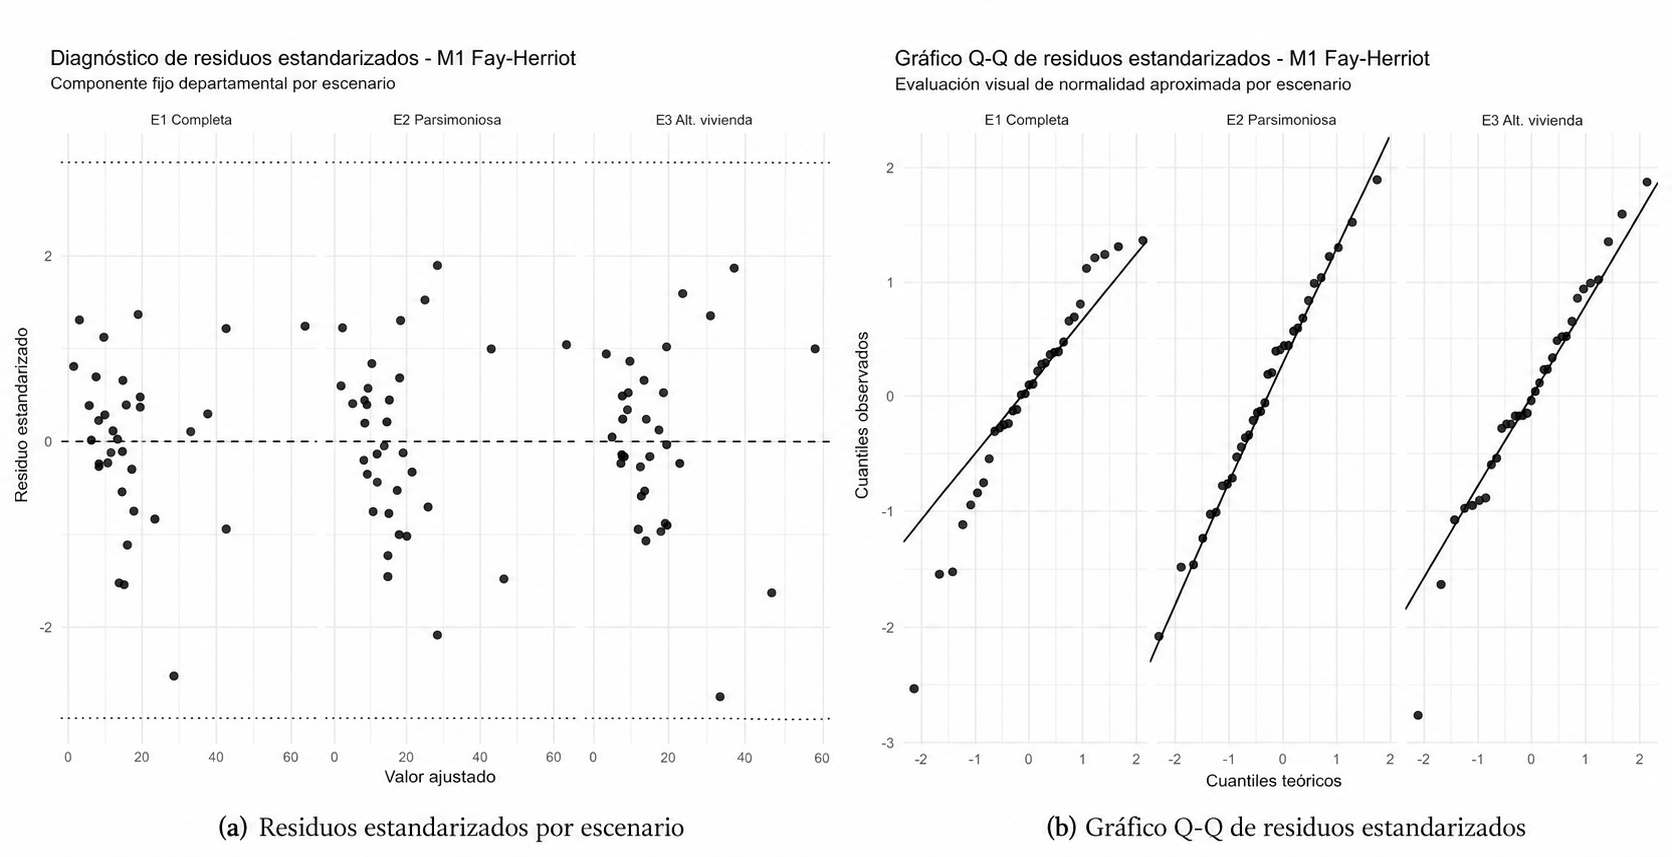
\includegraphics[width=0.95\textwidth]{fig/figures/Diagnósticos gráficos de residuos del modelo Fay–Herriot..png}
\caption{Diagnósticos gráficos de residuos del modelo Fay--Herriot.}
\label{fig:diag-M1}
\end{figure}

La evaluación formal de la validez interna incorporó diagnósticos relacionados con colinealidad entre covariables, adecuación de la forma funcional, heterocedasticidad, normalidad aproximada de los residuos estandarizados y presencia de dominios potencialmente influyentes. Los resultados se presentan en la Tabla~\ref{tab:fh-validez-interna}.

\begin{table}[!htbp]
\centering
\scriptsize
\caption{Diagnósticos de validez interna del modelo Fay--Herriot.}
\label{tab:fh-validez-interna}
\renewcommand{\arraystretch}{1.20}
\resizebox{\textwidth}{!}{
\begin{tabular}{l c c c c c c c}
\hline
\textbf{Escenario} &
\textbf{VIF máx.} &
\textbf{RESET $p$} &
\textbf{BP $p$} &
\textbf{Shapiro $p$} &
\textbf{$|r^{*}|>3$} &
\textbf{Dom. influyentes} &
\textbf{Estado} \\
\hline
Completo
& 5.005 & 0.0014 & 0.6672 & 0.1953 & 0 & 6
& Apto con advertencias \\

Parsimonioso
& 2.477 & 0.0898 & 0.0804 & 0.9965 & 0 & 7
& Apto con advertencias \\

Alt. vivienda
& 2.729 & 0.5292 & 0.0372 & 0.5821 & 0 & 6
& Apto con advertencias \\
\hline
\end{tabular}
}
\vspace{0.15cm}

\begin{minipage}{0.96\textwidth}
\footnotesize
\textit{Nota:} BP corresponde a la prueba de Breusch--Pagan y $r^{*}$ al residuo estandarizado. Los diagnósticos se interpretaron como señales de revisión y no como reglas automáticas de exclusión. La clasificación de aptitud estructural se basó en la validez de las varianzas directas, la no negatividad de $\sigma_u^2$, la finitud de los coeficientes estimados y la existencia de EBLUP finitos.
\end{minipage}
\end{table}

El escenario Completo concentró las principales advertencias relacionadas con la especificación del componente fijo. Su VIF máximo fue de 5.005, valor superior al observado en los otros dos escenarios, mientras que la prueba RESET resultó estadísticamente significativa ($p=0.0014$). Este resultado proporciona evidencia de posibles limitaciones en la forma funcional especificada y, por tanto, requiere cautela en su interpretación.

En contraste, los escenarios Parsimonioso y Alternativo de vivienda presentaron menores niveles de colinealidad, con VIF máximos de 2.477 y 2.729, respectivamente, y no mostraron evidencia estadísticamente significativa de problemas de especificación según la prueba RESET. En este sentido, ambos escenarios exhibieron un comportamiento más favorable respecto a la estructura del componente fijo.

En cuanto a la distribución de los residuos, la prueba de Shapiro--Wilk no proporcionó evidencia suficiente para rechazar el supuesto de normalidad aproximada en ninguno de los tres escenarios. De manera consistente, tampoco se identificaron residuos estandarizados con valores absolutos superiores a tres, lo que indica ausencia de observaciones extremadamente atípicas bajo este criterio.

La prueba de Breusch--Pagan tampoco mostró evidencia significativa de heterocedasticidad en los escenarios Completo y Parsimonioso. Sin embargo, en el escenario Alternativo de vivienda se obtuvo un valor $p=0.0372$, señalando posible heterocedasticidad. De acuerdo con los criterios establecidos en la metodología, este resultado se mantuvo como una advertencia diagnóstica y no constituyó por sí solo una condición automática de exclusión del escenario.

Adicionalmente, se identificaron dominios potencialmente influyentes en las tres especificaciones: seis en el escenario Completo, siete en el Parsimonioso y seis en el Alternativo de vivienda. La presencia de estos dominios justificó mantener su seguimiento durante las etapas posteriores de validación, especialmente al analizar la estabilidad de las estimaciones y el desempeño predictivo fuera de dominio.

En conjunto, los resultados de ajuste y diagnóstico muestran que los tres escenarios cumplieron las condiciones estructurales mínimas requeridas para el modelo Fay--Herriot y pudieron avanzar a la etapa de validación LODO. No obstante, ninguno se consideró completamente exento de advertencias. El escenario Completo presentó señales relacionadas principalmente con la forma funcional y la colinealidad, mientras que el escenario Alternativo de vivienda mostró evidencia de posible heterocedasticidad. Por esta razón, la selección y comparación posterior de las especificaciones no se sustentó exclusivamente en los criterios de ajuste interno, sino también en su capacidad predictiva fuera de dominio y en la coherencia global de las estimaciones.

\subsection{Desempeño predictivo departamental mediante LODO}

La capacidad predictiva fuera de dominio se evaluó excluyendo sucesivamente cada uno de los 33 departamentos y prediciéndolo a partir de los restantes. La Tabla~\ref{tab:fh-lodo} presenta las métricas obtenidas.

\begin{table}[!htbp]
\centering
\small
\caption{Desempeño predictivo LODO 2024 del modelo Fay--Herriot.}
\label{tab:fh-lodo}
\renewcommand{\arraystretch}{1.20}
\begin{tabular}{l c c c c}
\hline
\textbf{Escenario} &
\textbf{RMSE} &
\textbf{MAE} &
\textbf{Correlación} &
\textbf{$n$} \\
\hline
Completo          & 7.7047 & 5.2993 & 0.8316 & 33 \\
Parsimonioso      & 7.7563 & 5.9992 & 0.8303 & 33 \\
Alt. vivienda     & 7.8849 & 5.7569 & 0.8233 & 33 \\
\hline
\end{tabular}
\end{table}

Las diferencias de desempeño entre los tres escenarios fueron reducidas. El menor RMSE correspondió al escenario Completo, con 7.7047, seguido del Parsimonioso con 7.7563 y del Alternativo de vivienda con 7.8849. La diferencia entre el valor máximo y mínimo del RMSE fue de aproximadamente 0.18 puntos, lo que evidencia una baja sensibilidad del desempeño predictivo de M1 frente a los cambios en la especificación de covariables.

La misma estabilidad se observa en la correlación entre las estimaciones directas y las predicciones LODO, cuyos valores se ubicaron entre 0.8233 y 0.8316. Esta estabilidad no implica, sin embargo, que el modelo presente el menor error entre las tres familias evaluadas; la comparación entre M1, M2 y M3 se desarrolla posteriormente en la Sección~\ref{sec:res-comparacion}.

Debe distinguirse también el soporte de las predicciones obtenidas durante LODO del comportamiento de la proyección municipal completa. En la validación departamental, una predicción quedó fuera del intervalo 0--100 en el escenario Completo, una en el Parsimonioso y ninguna en el Alternativo de vivienda. Esta situación es independiente del número de proyecciones municipales fuera de rango, que se analiza a continuación.

\subsection{Proyección sintética municipal del IPM 2024}

Una vez ajustado el modelo departamental, se construyó una proyección sintética para los 1,121 municipios de la muestra analítica. Para cada municipio se aplicaron los coeficientes del componente fijo a sus covariables y se incorporó el efecto aleatorio estimado del departamento correspondiente. Esta operación permite trasladar la estructura calibrada a escala departamental hacia el nivel municipal, pero no modifica la naturaleza del modelo: M1 continúa siendo un modelo Fay--Herriot de área estimado con información directa departamental.

A diferencia de M2 y M3, la formulación lineal de M1 no incorpora una transformación que garantice por construcción que las proyecciones municipales permanezcan dentro del intervalo admisible del IPM. Esta limitación se hizo evidente en los tres escenarios, como se resume en la Tabla~\ref{tab:fh-proyeccion-municipal}.

\begin{table}[!htbp]
\centering
\small
\caption{Comportamiento del soporte de la proyección sintética municipal de M1.}
\label{tab:fh-proyeccion-municipal}
\renewcommand{\arraystretch}{1.20}
\begin{tabular}{l c c c c}
\hline
\textbf{Escenario} &
\textbf{$<0$} &
\textbf{$>100$} &
\textbf{Fuera de 0--100} &
\textbf{Total municipios} \\
\hline
Completo          & 197 & 2 & 199 & 1,121 \\
Parsimonioso      & 91  & 1 & 92  & 1,121 \\
Alt. vivienda     & 115 & 1 & 116 & 1,121 \\
\hline
\end{tabular}
\end{table}

El escenario Completo presentó la mayor cantidad de proyecciones municipales fuera del soporte del indicador, con 199 unidades, de las cuales 197 correspondieron a valores negativos y dos a valores superiores a 100. El escenario Parsimonioso redujo considerablemente esta situación, con 92 unidades fuera de rango, mientras que el Alternativo de vivienda presentó 116.

Estos valores no invalidan el ajuste Fay--Herriot a escala departamental, puesto que la estimación directa, la varianza de muestreo y los efectos aleatorios se definieron en ese nivel. No obstante, sí constituyen una limitación relevante de la utilización del predictor lineal como mecanismo de desagregación hacia municipios y justifican que el cumplimiento del soporte 0--100 sea evaluado explícitamente al comparar M1 con las formulaciones no lineales.

Para la comparación municipal común entre los tres modelos se utilizó el escenario Parsimonioso. Las proyecciones originales de M1 se conservaron para los análisis cuantitativos y para documentar las observaciones fuera de rango; cualquier acotamiento aplicado en la representación cartográfica tuvo únicamente fines de visualización y no alteró los valores utilizados en la evaluación estadística.

En síntesis, M1 mostró una elevada estabilidad predictiva frente a los cambios de escenario y cumplió las condiciones estructurales requeridas para el ajuste departamental. Sin embargo, la presencia de dominios influyentes y, especialmente, la existencia de proyecciones sintéticas municipales fuera del rango admisible muestran que la extrapolación del modelo de área hacia la escala municipal debe interpretarse con cautela. Estas propiedades se consideran conjuntamente con el desempeño de M2 y M3 en la comparación integrada presentada posteriormente.

%--------------------------------------------------------------------------------------
\section{Implementación del Modelo 2: desagregación municipal no lineal acotada}
\label{sec:res-m2}

El modelo M2 genera las predicciones a escala municipal mediante una transformación logística aplicada directamente sobre las covariables de cada municipio. Sin embargo, la calibración de sus parámetros se realiza utilizando como referencia las 33 estimaciones directas departamentales, obtenidas al agregar las predicciones municipales mediante los pesos poblacionales definidos en la metodología. En consecuencia, la información auxiliar entra al modelo a escala municipal, mientras que la función de verosimilitud y la validación predictiva se evalúan a escala departamental.

Esta formulación se diferencia de M1 en dos aspectos principales. En primer lugar, la transformación logística garantiza por construcción que las estimaciones municipales permanezcan dentro del intervalo admisible del IPM. En segundo lugar, el procedimiento de \textit{benchmarking} permite que, en el ajuste final, el promedio ponderado de las estimaciones municipales reproduzca numéricamente la estimación directa de cada departamento.

\subsection{Ajuste y validez interna}

Los tres escenarios alcanzaron convergencia satisfactoria y presentaron parámetros finitos. La estimación se realizó a partir de 12 puntos iniciales para cada especificación; en los tres casos, los 12 arranques fueron válidos y convergieron hacia el mismo óptimo dentro de la tolerancia establecida. Asimismo, la matriz Hessiana resultó definida positiva en las tres especificaciones, lo que aporta evidencia favorable sobre la identificación local de las soluciones obtenidas.

La desviación estándar adicional, $\tau$, presentó valores de 3.2095 en el escenario Completo, 4.5708 en el Parsimonioso y 5.3426 en el Alternativo de vivienda. Estos valores corresponden a la componente adicional de variabilidad incorporada en la función de verosimilitud, cuya varianza entra al modelo como $\tau^2$.

La Tabla~\ref{tab:m2-validez-interna} resume los principales diagnósticos de validez interna.

\begin{table}[!htbp]
\centering
\scriptsize
\caption{Diagnósticos de validez interna del modelo no lineal acotado.}
\label{tab:m2-validez-interna}
\renewcommand{\arraystretch}{1.20}
\resizebox{\textwidth}{!}{
\begin{tabular}{l c c c c c c c c}
\hline
\textbf{Escenario} &
\textbf{$\tau$} &
\textbf{Arranques válidos} &
\textbf{Hessiano PD} &
\textbf{Dom./par.} &
\textbf{Shapiro $p$} &
\textbf{$|r^{*}|>3$} &
\textbf{Benchmarking} &
\textbf{Estado} \\
\hline
Completo
& 3.2095 & 12/12 & Sí & 3.67 & 0.2883 & 0
& $3.45\times10^{-12}$
& Apto con advertencias \\

Parsimonioso
& 4.5708 & 12/12 & Sí & 5.50 & 0.1437 & 0
& $3.28\times10^{-12}$
& Apto \\

Alt. vivienda
& 5.3426 & 12/12 & Sí & 5.50 & 0.0813 & 1
& $5.04\times10^{-12}$
& Apto con advertencias \\
\hline
\end{tabular}
}

\vspace{0.15cm}
\begin{minipage}{0.96\textwidth}
\footnotesize
\textit{Nota:} PD indica que la matriz Hessiana fue definida positiva; Dom./par. corresponde a la razón entre dominios y parámetros estimados; $r^{*}$ representa el residuo departamental estandarizado previo al \textit{benchmarking}. El error de \textit{benchmarking} corresponde a la máxima diferencia absoluta entre el IPM directo departamental y el agregado ponderado de las estimaciones municipales ajustadas.
\end{minipage}
\end{table}

El escenario Completo fue clasificado como apto con advertencias debido a que la razón entre dominios y parámetros fue de 3.67, inferior al umbral de cinco dominios por parámetro utilizado como criterio diagnóstico. Esta situación refleja la mayor carga paramétrica de E1 frente al número limitado de observaciones departamentales disponibles para la calibración.

El escenario Parsimonioso no presentó advertencias internas. Los 12 arranques produjeron soluciones estables, la matriz Hessiana fue definida positiva, no se identificaron residuos estandarizados superiores a tres y la razón entre dominios y parámetros fue de 5.50.

El escenario Alternativo de vivienda también cumplió las condiciones estructurales del ajuste, aunque se identificó un residuo departamental pre-\textit{benchmarking} con valor absoluto superior a tres. La prueba de Shapiro--Wilk aplicada al conjunto de residuos estandarizados no resultó significativa ($p=0.0813$), por lo que la advertencia se interpretó como un resultado localizado y no como evidencia suficiente para descartar la especificación.

En las tres formulaciones, las covariables presentaron variación suficiente, los parámetros estimados fueron finitos y la transformación logística mantuvo todas las predicciones dentro del intervalo 0--100. Además, el error máximo de \textit{benchmarking} se ubicó en el orden de $10^{-12}$, lo que indica que la restricción de coherencia departamental se cumplió dentro de la precisión numérica del procedimiento.

La Tabla~\ref{tab:m2-soporte} presenta el rango de las estimaciones municipales finales después del \textit{benchmarking}.

\begin{table}[!htbp]
\centering
\small
\caption{Rango y coherencia de las estimaciones municipales finales de M2.}
\label{tab:m2-soporte}
\renewcommand{\arraystretch}{1.20}
\begin{tabular}{l c c c c}
\hline
\textbf{Escenario} &
\textbf{Mínimo} &
\textbf{Máximo} &
\textbf{Fuera de 0--100} &
\textbf{Error de benchmarking} \\
\hline
Completo          & 0.120 & 99.081 & 0 & $3.45\times10^{-12}$ \\
Parsimonioso      & 1.547 & 98.008 & 0 & $3.28\times10^{-12}$ \\
Alt. vivienda     & 2.360 & 97.462 & 0 & $5.04\times10^{-12}$ \\
\hline
\end{tabular}
\end{table}

Estos resultados muestran una diferencia estructural frente a M1: ninguna de las estimaciones municipales generadas por M2 requirió truncamiento posterior para respetar el soporte del IPM.

\subsection{Desempeño predictivo departamental mediante LODO}

La capacidad predictiva fuera de dominio se evaluó mediante la misma estrategia LODO aplicada a M1. En cada iteración se excluyó un departamento completo del ajuste, las covariables se estandarizaron nuevamente utilizando únicamente los municipios de entrenamiento y el dominio excluido no recibió \textit{benchmarking}. Esta última condición es fundamental, ya que aplicar el ajuste de coherencia al departamento de evaluación implicaría utilizar su propia estimación directa para construir la predicción.

Los resultados se presentan en la Tabla~\ref{tab:m2-lodo}.

\begin{table}[!htbp]
\centering
\small
\caption{Desempeño predictivo LODO 2024 del modelo no lineal acotado.}
\label{tab:m2-lodo}
\renewcommand{\arraystretch}{1.20}
\begin{tabular}{l c c c c}
\hline
\textbf{Escenario} &
\textbf{RMSE} &
\textbf{MAE} &
\textbf{Correlación} &
\textbf{$n$} \\
\hline
Completo          & 5.0971 & 3.7048 & 0.9301 & 33 \\
Parsimonioso      & 6.4540 & 4.8405 & 0.8855 & 33 \\
Alt. vivienda     & 8.4065 & 5.6452 & 0.7964 & 33 \\
\hline
\end{tabular}
\end{table}

Dentro de la familia M2, el escenario Completo presentó el menor error predictivo, con RMSE de 5.0971 y MAE de 3.7048, además de la mayor correlación entre estimaciones directas y predicciones LODO, con un valor de 0.9301. El escenario Parsimonioso presentó un desempeño intermedio, con RMSE de 6.4540, MAE de 4.8405 y correlación de 0.8855.

El escenario Alternativo de vivienda presentó el mayor error dentro de M2, con RMSE de 8.4065 y MAE de 5.6452, acompañado por una correlación inferior, de 0.7964. La diferencia entre el mayor y el menor RMSE fue de aproximadamente 3.31 puntos, lo que evidencia una sensibilidad más alta a la selección de covariables que la observada en M1.

Este resultado muestra que la mayor parsimonia no se tradujo automáticamente en un menor error predictivo dentro de M2. No obstante, la comparación entre familias de modelos se reserva para la Sección~\ref{sec:res-comparacion}, dado que el objetivo aquí es caracterizar el comportamiento interno de la formulación no lineal.

\subsection{Estimación municipal del IPM 2024}

Una vez completado el ajuste con los 33 dominios, se generaron estimaciones finales para los 1,121 municipios de la muestra analítica. A diferencia de M1, estas estimaciones se construyen directamente a partir del predictor municipal transformado mediante la función logística, por lo que el soporte del indicador se encuentra garantizado por la propia especificación funcional.

Posteriormente se aplicó el procedimiento de \textit{benchmarking} mediante un desplazamiento departamental en la escala del predictor. Este ajuste permitió que el promedio ponderado de las estimaciones municipales coincidiera, dentro de la precisión numérica, con el IPM directo del departamento correspondiente sin alterar la propiedad de acotamiento.

Por esta razón, el \textit{benchmarking} debe interpretarse como un procedimiento de coherencia estructural de la estimación final y no como evidencia de capacidad predictiva. La capacidad de generalización del modelo se evaluó de manera independiente mediante LODO, donde el departamento excluido no recibió este ajuste.

Para la comparación municipal común con M1 y M3 se utilizó el escenario Parsimonioso. Bajo esta especificación, las estimaciones municipales de M2 se ubicaron entre 1.547 y 98.008 puntos del IPM y no se presentaron valores fuera del intervalo admisible.

La comparación posterior con M3 bajo el mismo escenario mostró una correlación municipal de 0.9901 y una diferencia absoluta media de 1.69 puntos porcentuales. Estas medidas se interpretan como indicadores de concordancia entre formulaciones y no como métricas de precisión municipal, dado que no se dispone de una estimación directa municipal del IPM 2024 que pueda utilizarse como referencia observada.

En síntesis, M2 presentó estabilidad numérica en los tres escenarios, cumplimiento exacto de las restricciones de soporte y coherencia departamental, y un desempeño predictivo que varió de manera apreciable según la especificación de covariables. El escenario Completo alcanzó el menor error LODO dentro de esta familia, mientras que el escenario Parsimonioso presentó la estructura interna más limpia al no registrar advertencias diagnósticas. Estas diferencias se incorporan posteriormente en la comparación integrada de las tres formulaciones.
%--------------------------------------------------------------------------------------
\section{Implementación del Modelo 3: desagregación espacial CAR}
\label{sec:res-m3}

El modelo M3 extiende la formulación no lineal acotada de M2 mediante la incorporación de un componente espacial municipal con estructura condicional autorregresiva (CAR) de rango reducido. Al igual que en M2, las covariables ingresan al modelo a escala municipal, las predicciones se transforman mediante una función logística y la calibración de los parámetros se realiza utilizando como referencia las 33 estimaciones directas departamentales.

La principal diferencia respecto a M2 radica en la inclusión de un efecto espacial construido a partir de la estructura de vecindad municipal. Este componente se representó mediante seis patrones espaciales de rango reducido, obtenidos a partir de la matriz de contigüidad tipo Reina, con el propósito de incorporar dependencia territorial sin estimar un efecto independiente para cada uno de los 1,121 municipios.

\subsection{Ajuste, validez interna y sensibilidad espacial}

Durante las etapas preliminares de estimación del modelo espacial CAR de rango reducido (M3) se exploró la estimación libre del parámetro de dependencia espacial, $\rho$. Sin embargo, las soluciones obtenidas se concentraron repetidamente en los límites del intervalo de búsqueda: inicialmente alrededor de $-0.95$ y, posteriormente, cerca de $0.95$ bajo una parametrización alternativa. Este comportamiento sugirió una identificación limitada de $\rho$ cuando su estimación se sustenta únicamente en la información agregada de los 33 dominios departamentales utilizados para la calibración.

En consecuencia, se optó por tratar $\rho$ como un parámetro de sensibilidad en lugar de estimarlo libremente dentro del modelo final. Para ello, se evaluaron cuatro valores predefinidos:

\[
\rho \in \{0.25,\;0.50,\;0.75,\;0.90\}.
\]

Se estableció $\rho=0.50$ como especificación de referencia para la comparación principal de M3, mientras que los demás valores se utilizaron para examinar la estabilidad de los parámetros estimados y de las predicciones municipales frente a distintos niveles de dependencia espacial impuesta.

Bajo la especificación de referencia, los tres escenarios considerados alcanzaron convergencia satisfactoria. Para cada escenario se utilizaron ocho puntos iniciales y, en todos los casos, los ocho arranques fueron válidos y convergieron hacia el mismo óptimo dentro de la tolerancia establecida. Asimismo, la matriz Hessiana resultó definida positiva y la matriz de precisión asociada a la estructura CAR permaneció válida, proporcionando evidencia favorable sobre la estabilidad numérica de la estimación.

La Tabla~\ref{tab:m3-validez-interna} resume los principales diagnósticos internos obtenidos para el modelo espacial con $\rho=0.50$.

\begin{table}[!htbp]
\centering
\scriptsize
\caption{Diagnósticos de validez interna del modelo espacial CAR de rango reducido con $\rho=0.50$.}
\label{tab:m3-validez-interna}
\renewcommand{\arraystretch}{1.20}
\resizebox{\textwidth}{!}{
\begin{tabular}{l c c c c c c c c}
\hline
\textbf{Escenario} &
\textbf{$\tau$} &
\textbf{DE efecto espacial} &
\textbf{Moran $I$} &
\textbf{$p$ Moran} &
\textbf{Arranques válidos} &
\textbf{Hessiano PD} &
\textbf{$|r^{*}|>3$} &
\textbf{Estado} \\
\hline
Completo
& 2.0993 & 0.2501 & 0.9883 & 0.001
& 8/8 & Sí & 0
& Apto con advertencias \\

Parsimonioso
& 2.5584 & 0.3257 & 0.9935 & 0.001
& 8/8 & Sí & 0
& Apto con advertencias \\

Alt. vivienda
& 3.9040 & 0.3391 & 0.9966 & 0.001
& 8/8 & Sí & 0
& Apto con advertencias \\
\hline
\end{tabular}
}

\vspace{0.15cm}
\begin{minipage}{0.96\textwidth}
\footnotesize
\textit{Nota:} PD indica que la matriz Hessiana fue definida positiva; DE corresponde a la desviación estándar del efecto espacial municipal; $r^{*}$ representa el residuo departamental estandarizado previo al \textit{benchmarking}. El estadístico global de Moran se calculó sobre el efecto espacial municipal estimado y no sobre los residuos finales del modelo.
\end{minipage}
\end{table}

La desviación estándar departamental adicional, $\tau$, fue de 2.0993 en el escenario Completo, 2.5584 en el escenario Parsimonioso y 3.9040 en el escenario Alternativo de vivienda. Este incremento indica que, bajo las especificaciones más reducidas, una mayor proporción de la variabilidad departamental no explicada por las covariables debió ser absorbida por el componente aleatorio adicional del modelo.

De manera similar, la desviación estándar del efecto espacial municipal aumentó desde 0.2501 en el escenario Completo hasta 0.3391 en el Alternativo de vivienda. Estas diferencias reflejan variaciones en la magnitud del componente territorial requerido por cada especificación para representar la heterogeneidad espacial no capturada por el componente fijo.

El efecto espacial estimado presentó una autocorrelación positiva elevada en los tres escenarios. El índice global de Moran varió entre 0.9883 y 0.9966, con valores $p=0.001$ en todos los casos. Este resultado indica que el componente espacial retenido por la representación CAR de rango reducido conserva una estructura geográfica fuertemente organizada y coherente con la matriz de vecindad utilizada en el modelo.

No obstante, estos valores deben interpretarse con cautela. El índice de Moran fue calculado sobre el propio efecto espacial estimado y, por tanto, no constituye una prueba de ausencia de autocorrelación en los residuos finales. Su función en este contexto es caracterizar la organización espacial del componente territorial incorporado por el modelo, mientras que la evaluación de la autocorrelación residual corresponde a un diagnóstico diferente.

La Figura~\ref{fig:diag-Moran} presenta gráficamente esta relación mediante el diagrama de Moran del efecto espacial municipal estimado.

\begin{figure}[!htbp]
\centering
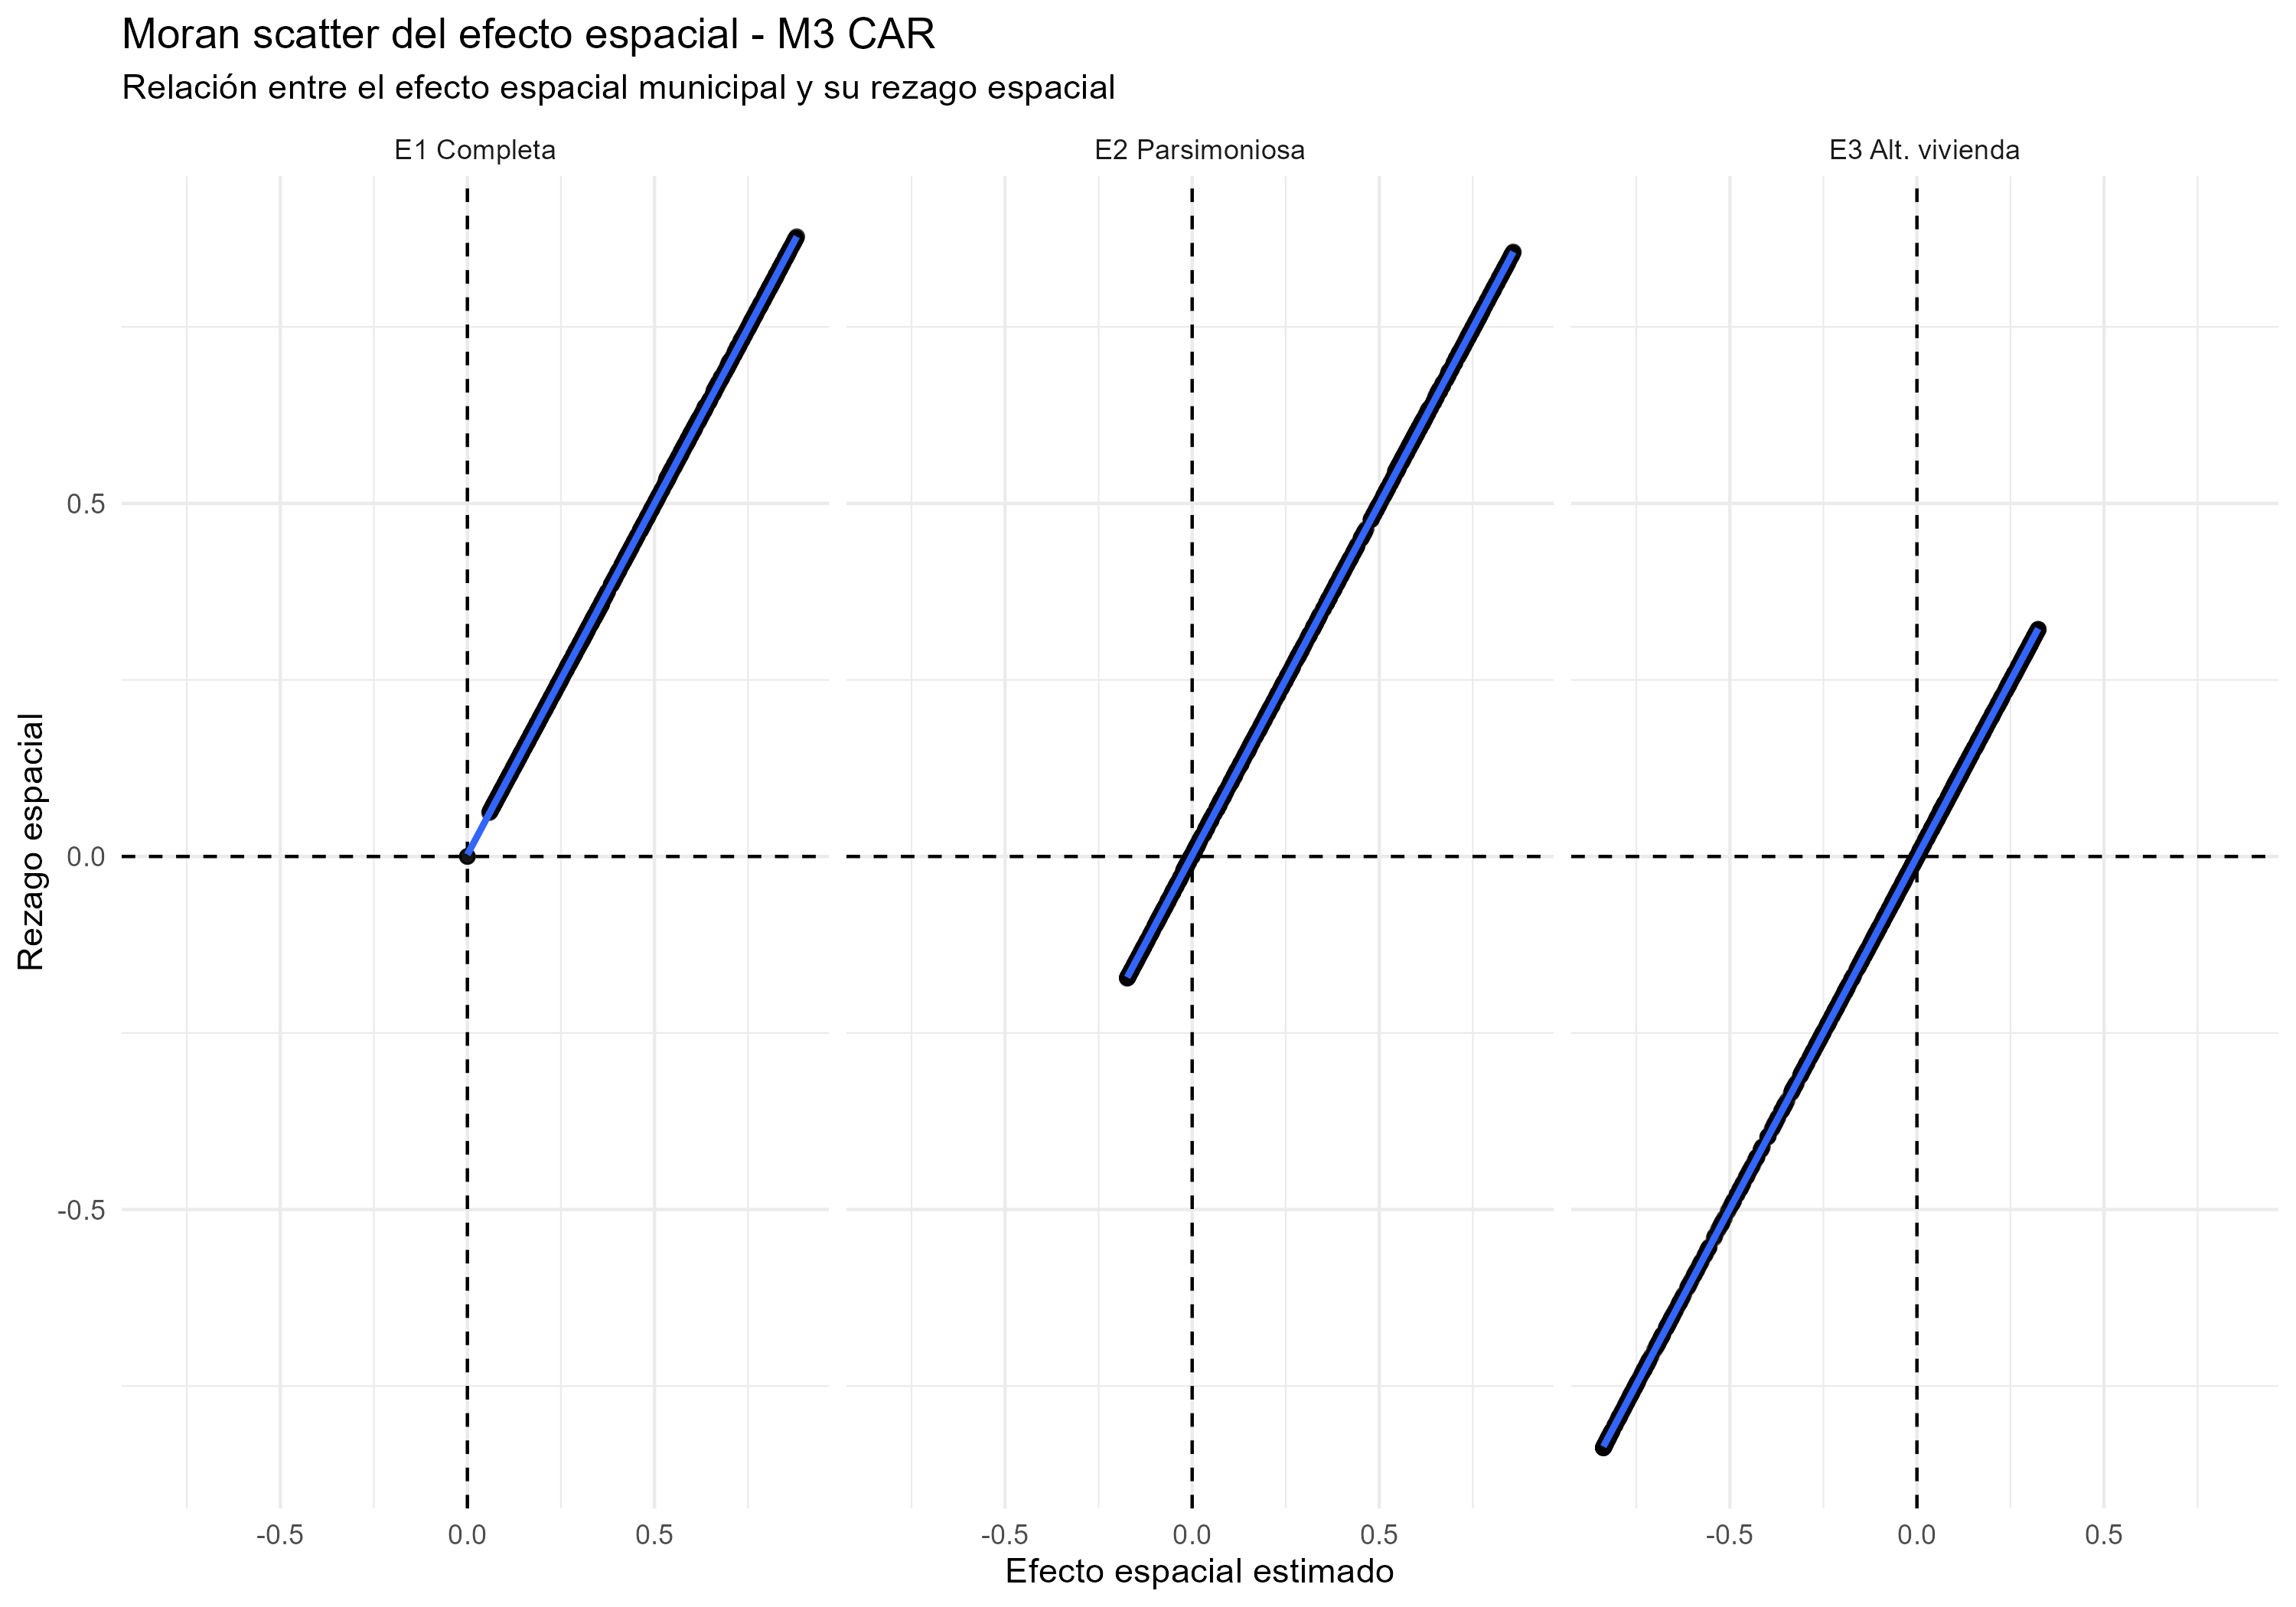
\includegraphics[width=0.95\textwidth]{fig/figures/diagnostico_M3_Moran_efecto_espacial.png}
\caption{Diagrama de Moran del efecto espacial municipal estimado por el modelo CAR.}
\label{fig:diag-Moran}
\end{figure}

En relación con los residuos departamentales previos al \textit{benchmarking}, no se identificaron valores estandarizados con valor absoluto superior a tres en ninguno de los escenarios. Este resultado indica que, bajo este criterio, no se observaron desviaciones extremas en los residuos utilizados para evaluar la consistencia interna del ajuste.

Las principales advertencias asociadas a M3 estuvieron relacionadas con la estructura de la red espacial municipal. Bajo el criterio de contigüidad tipo Reina, dos unidades insulares no presentaron vecinos directos y la red espacial quedó conformada inicialmente por tres componentes conexos. Estas particularidades, descritas previamente en la sección de preprocesamiento espacial, fueron tratadas explícitamente durante la construcción de la matriz de vecindad y se conservaron como advertencias metodológicas. Su presencia no implicó la eliminación de municipios ni la modificación del universo de estimación.

Con base en estos resultados, los tres escenarios cumplieron las condiciones mínimas de validez interna definidas para el modelo M3. La convergencia consistente entre múltiples puntos iniciales, la existencia de Hessianos definidos positivos, la validez de la matriz de precisión espacial y la ausencia de residuos departamentales extremos proporcionaron evidencia favorable sobre la estabilidad del procedimiento de estimación, aunque las particularidades de conectividad de la red espacial justificaron mantener la clasificación de ``apto con advertencias''.

Finalmente, se evaluó la sensibilidad de los resultados frente al valor fijado de $\rho$. Al variar el parámetro entre 0.25 y 0.90, los cambios observados en $\tau$, en la desviación estándar del efecto espacial y en los valores extremos de las predicciones municipales fueron reducidos. Asimismo, las estimaciones municipales se mantuvieron dentro del intervalo teórico de 0 a 100 para todos los valores analizados.

El procedimiento de \textit{benchmarking} también conservó su exactitud numérica en toda la grilla de sensibilidad. En consecuencia, los principales resultados de M3 mostraron estabilidad frente a variaciones moderadas y altas del parámetro $\rho$ dentro del rango evaluado. Esto respalda el uso de $\rho=0.50$ como especificación de referencia para la comparación principal, sin interpretar dicho valor como una estimación empírica única o identificada directamente a partir de los datos.

\subsection{Desempeño predictivo departamental mediante LODO}

La capacidad predictiva fuera de dominio se evaluó mediante la misma estrategia LODO utilizada para M1 y M2. En cada iteración, el departamento excluido no participó en la estimación de los parámetros ni recibió \textit{benchmarking}. La estandarización de las covariables se recalculó utilizando únicamente los municipios pertenecientes a los dominios de entrenamiento.

La información geográfica y la estructura de vecindad del dominio excluido permanecieron disponibles durante la predicción, dado que constituyen información auxiliar externa y no forman parte de la respuesta directa utilizada para la evaluación.

Los resultados de la validación se presentan en la Tabla~\ref{tab:m3-lodo}.

\begin{table}[!htbp]
\centering
\small
\caption{Desempeño predictivo LODO 2024 del modelo espacial CAR de rango reducido con $\rho=0.50$.}
\label{tab:m3-lodo}
\renewcommand{\arraystretch}{1.20}
\begin{tabular}{l c c c c}
\hline
\textbf{Escenario} &
\textbf{RMSE} &
\textbf{MAE} &
\textbf{Correlación} &
\textbf{$n$} \\
\hline
Completo          & 6.0406  & 4.4623 & 0.9001 & 33 \\
Parsimonioso      & 4.7197  & 3.6731 & 0.9410 & 33 \\
Alt. vivienda     & 10.4274 & 6.5350 & 0.7063 & 33 \\
\hline
\end{tabular}
\end{table}

Dentro de la familia M3, el escenario Parsimonioso presentó el menor error predictivo, con un RMSE de 4.7197 y un MAE de 3.6731, acompañado por la mayor correlación entre las estimaciones directas y las predicciones LODO, con un valor de 0.9410.

El escenario Completo mostró un desempeño intermedio, con RMSE de 6.0406, MAE de 4.4623 y correlación de 0.9001. En contraste, el escenario Alternativo de vivienda presentó un deterioro importante del desempeño predictivo, alcanzando un RMSE de 10.4274, un MAE de 6.5350 y una correlación de 0.7063.

La diferencia entre el mayor y el menor RMSE fue aproximadamente de 5.71 puntos, la mayor variación observada entre escenarios dentro de las tres familias de modelos. Este resultado indica que la formulación espacial es particularmente sensible al conjunto de covariables utilizado y que la incorporación de dependencia espacial no compensa automáticamente una especificación auxiliar menos favorable.

La comparación directa de este desempeño con M1 y M2 se presenta posteriormente en la Sección~\ref{sec:res-comparacion}, con el propósito de mantener separada la evaluación interna de M3 de la comparación integrada entre formulaciones.

\subsection{Estimación municipal del IPM 2024}

Una vez completada la calibración con los 33 dominios departamentales, se obtuvieron estimaciones para los 1,121 municipios de la muestra analítica. Al igual que en M2, el predictor municipal se transformó mediante una función logística, por lo que las estimaciones permanecieron dentro del intervalo admisible del IPM.

Para la estimación final se utilizó el escenario Parsimonioso con $\rho=0.50$, especificación adoptada como referencia común para la comparación municipal entre M1, M2 y M3. Posteriormente se aplicó el mismo procedimiento de \textit{benchmarking} utilizado en M2, mediante un desplazamiento departamental sobre la escala del predictor.

Después de este ajuste, las estimaciones municipales bajo E2 se ubicaron aproximadamente entre 0.96 y 99.20 puntos del IPM. No se identificaron valores inferiores a cero ni superiores a 100 y el agregado ponderado de las estimaciones municipales reprodujo, dentro de la precisión numérica, el IPM directo correspondiente a cada departamento.

Al igual que en M2, el \textit{benchmarking} se interpreta exclusivamente como una condición de coherencia estructural de la estimación final y no como evidencia de capacidad predictiva. La evaluación de generalización del modelo corresponde a los resultados LODO obtenidos sin utilizar la estimación directa del departamento excluido.

Bajo el escenario Parsimonioso, M3 presentó una elevada concordancia con las estimaciones municipales de M2. La correlación entre ambas formulaciones fue de 0.9901 y la diferencia absoluta media alcanzó 1.69 puntos porcentuales. La correlación entre M3 y la proyección sintética municipal de M1 fue de 0.9374. Estas medidas describen la similitud entre las distribuciones municipales producidas por los modelos, pero no constituyen medidas de precisión municipal.

En síntesis, M3 presentó estabilidad numérica en los tres escenarios, una estructura espacial claramente definida, cumplimiento del soporte 0--100 y coherencia departamental mediante \textit{benchmarking}. Su desempeño predictivo, sin embargo, mostró una sensibilidad considerable a la especificación de covariables: el escenario Parsimonioso presentó el menor error dentro de la familia, mientras que el Alternativo de vivienda mostró un deterioro sustancial. Estos resultados evidencian que el aporte del componente espacial depende de su interacción con la información auxiliar incorporada y deben interpretarse conjuntamente con las otras dos formulaciones en la comparación integrada.
%--------------------------------------------------------------------------------------
\section{Comparación integrada y producción cartográfica}
\label{sec:res-comparacion}

Una vez caracterizadas por separado las propiedades internas y el desempeño predictivo de M1, M2 y M3, se realizó una comparación integrada bajo condiciones comunes. Las nueve combinaciones de modelo y escenario superaron las condiciones mínimas establecidas para participar en esta etapa: completaron los 33 dominios de la validación \textit{Leave-One-Domain-Out} (LODO) y produjeron métricas de evaluación finitas.

Para garantizar la comparabilidad entre formulaciones, el RMSE, el MAE y la correlación LODO se calcularon sobre exactamente los mismos 33 dominios departamentales y mediante la misma estrategia de exclusión sucesiva en las nueve combinaciones evaluadas. En cada iteración, la estimación directa del departamento excluido permaneció fuera del proceso de ajuste y no se utilizó para construir su predicción.

La comparación entre familias se realizó exclusivamente con las métricas obtenidas mediante el mismo esquema LODO 2024. Los criterios de ajuste interno, como AIC, BIC o la función objetivo penalizada, no se utilizaron para ordenar modelos pertenecientes a familias probabilísticas diferentes, sino únicamente como diagnósticos internos de las especificaciones correspondientes.

\subsection{Comparación del desempeño predictivo}

La Tabla~\ref{tab:comparacion-m123} consolida el RMSE, MAE y la correlación entre las estimaciones directas departamentales y las predicciones LODO obtenidas para las nueve combinaciones evaluadas.

\begin{table}[!htbp]
\centering
\small
\caption{Comparación controlada del desempeño predictivo de M1, M2 y M3 mediante LODO 2024.}
\label{tab:comparacion-m123}
\renewcommand{\arraystretch}{1.20}
\begin{tabular}{l l c c c}
\hline
\textbf{Escenario} &
\textbf{Modelo} &
\textbf{RMSE} &
\textbf{MAE} &
\textbf{Correlación} \\
\hline
Completo
& M1 Fay--Herriot
& 7.7047 & 5.2993 & 0.8316 \\

Completo
& M2 no lineal
& 5.0971 & 3.7048 & 0.9301 \\

Completo
& M3 CAR
& 6.0406 & 4.4623 & 0.9001 \\
\hline
Parsimonioso
& M1 Fay--Herriot
& 7.7563 & 5.9992 & 0.8303 \\

Parsimonioso
& M2 no lineal
& 6.4540 & 4.8405 & 0.8855 \\

Parsimonioso
& M3 CAR
& 4.7197 & 3.6731 & 0.9410 \\
\hline
Alt. vivienda
& M1 Fay--Herriot
& 7.8849 & 5.7569 & 0.8233 \\

Alt. vivienda
& M2 no lineal
& 8.4065 & 5.6452 & 0.7964 \\

Alt. vivienda
& M3 CAR
& 10.4274 & 6.5350 & 0.7063 \\
\hline
\end{tabular}
\end{table}

La comparación por escenario muestra que ninguna familia presentó sistemáticamente el menor error bajo todas las especificaciones de covariables. En el escenario Completo, M2 alcanzó el menor RMSE (5.0971), seguido por M3 (6.0406) y M1 (7.7047). Bajo el escenario Parsimonioso, M3 presentó el menor RMSE de las nueve combinaciones evaluadas (4.7197), acompañado por el menor MAE (3.6731) y la mayor correlación LODO (0.9410). En el escenario Alternativo de vivienda, M1 presentó el menor RMSE (7.8849), aunque las diferencias con M2 fueron más reducidas que las observadas frente a M3.

Por tanto, la incorporación de un componente espacial no produjo una mejora automática del desempeño predictivo. Su aporte dependió de la interacción entre la estructura espacial y el conjunto de covariables utilizado. En particular, M3 mostró un comportamiento favorable bajo el escenario Parsimonioso, pero un deterioro considerable bajo el Alternativo de vivienda.

La combinación M3--Parsimonioso redujo el RMSE aproximadamente en un 7.4\,\% respecto a M2--Completo, que presentó el segundo menor RMSE entre las nueve combinaciones. Esta diferencia se interpreta como una comparación descriptiva del desempeño predictivo observado y no como evidencia suficiente, por sí sola, para seleccionar una formulación únicamente a partir de una métrica.

Las diferencias en el desempeño predictivo entre modelos y escenarios se presentan visualmente en los gráficos de la figura~\ref{fig:comparacion-desmp-predict}. Cada figura muestra, respectivamente, el RMSE, el MAE y la correlación obtenidos mediante la validación LODO para las nueve combinaciones evaluadas, facilitando la comparación tanto entre formulaciones como entre escenarios de covariables.

\begin{figure}[!htbp]
\centering
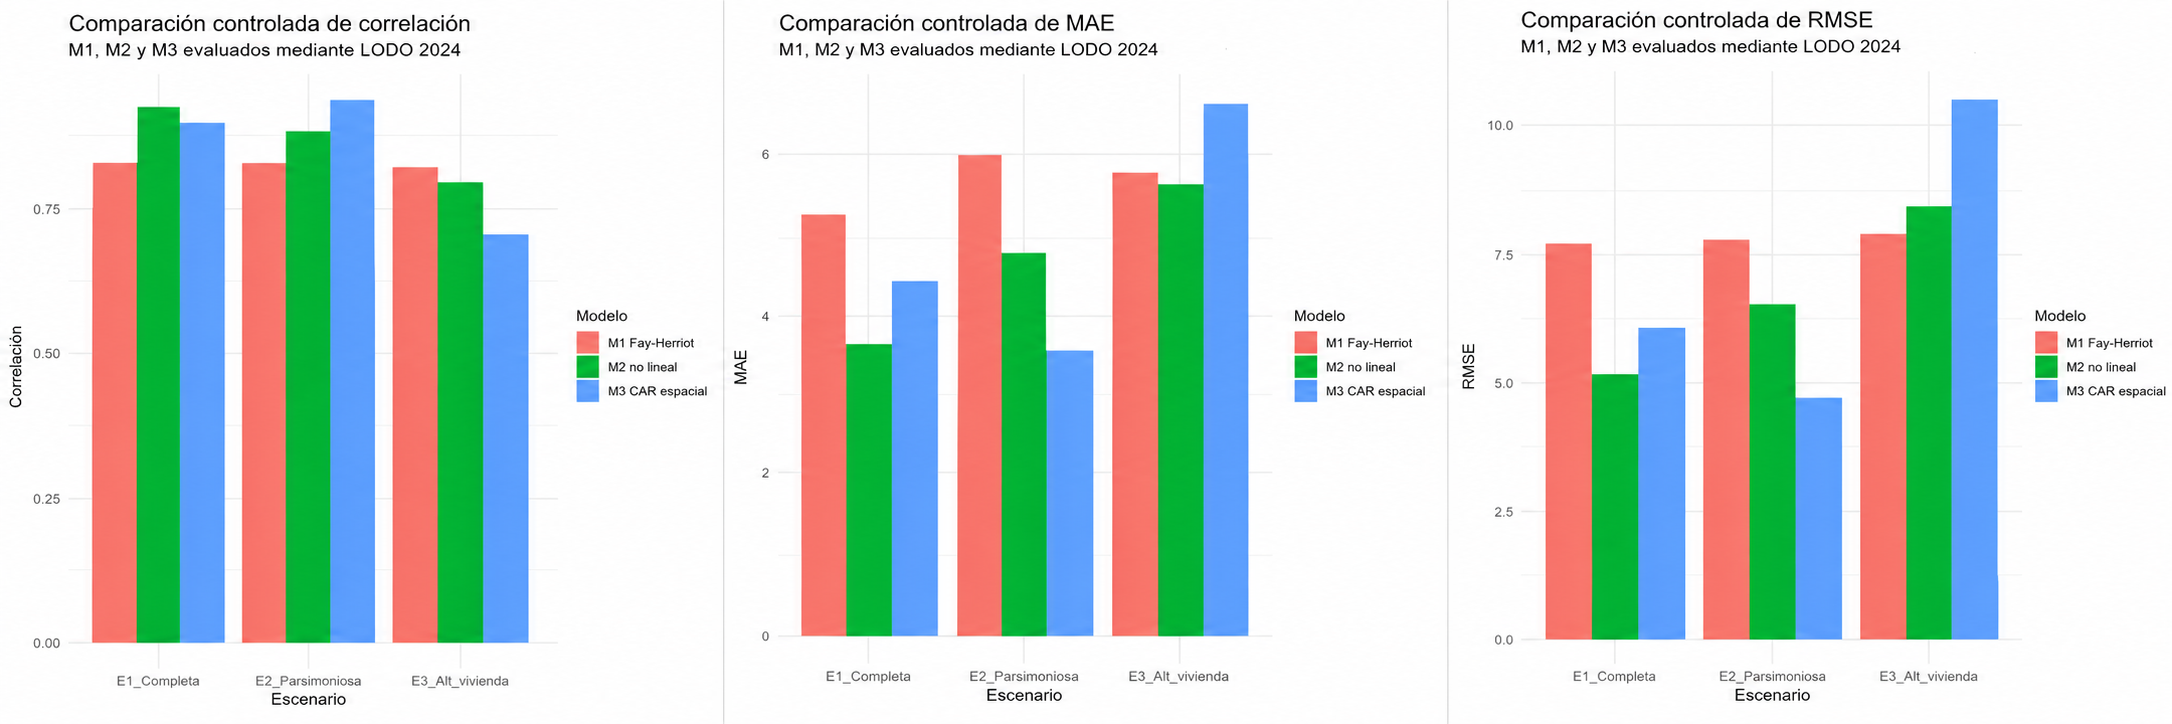
\includegraphics[width=0.95\textwidth]{fig/figures/Comparacion_Desemp_predict.png}
\caption{Comparación del desempeño predictivo de los modelos M1, M2 y M3.}
\label{fig:comparacion-desmp-predict}
\end{figure}

\subsection{Estabilidad frente a los escenarios de covariables}

Además del nivel de error, se examinó la estabilidad de cada familia frente a los cambios en la especificación auxiliar. M1 presentó la menor amplitud de RMSE entre escenarios, con una diferencia de 0.18 puntos entre su valor mínimo y máximo. En M2, esta amplitud aumentó a 3.31 puntos, mientras que M3 alcanzó 5.71 puntos.

Estos resultados muestran que M1 fue relativamente estable frente a las modificaciones del conjunto de covariables, aunque presentó un nivel de error LODO comparativamente similar en los tres escenarios. M2 mostró una sensibilidad intermedia, mientras que M3 presentó la mayor dependencia respecto a la especificación auxiliar.

Tomando únicamente el menor RMSE dentro de cada familia como resumen descriptivo, las formulaciones de referencia fueron el escenario Completo para M1 (RMSE = 7.7047), el escenario Completo para M2 (RMSE = 5.0971) y el escenario Parsimonioso para M3 (RMSE = 4.7197). Esta identificación se utiliza para describir el comportamiento interno de cada familia y no implica que un único escenario deba adoptarse como referencia para todas las comparaciones posteriores.

La comparación integrada también mostró diferencias en las propiedades garantizadas por cada formulación. M1 se estimó como un modelo Fay--Herriot a escala departamental y posteriormente produjo una proyección sintética municipal. Debido a su estructura lineal, esta proyección no garantiza el soporte 0--100 del IPM: en el ajuste final se identificaron 199, 92 y 116 proyecciones municipales fuera de rango bajo los escenarios Completo, Parsimonioso y Alternativo de vivienda, respectivamente.

M2 y M3, en cambio, incorporaron una transformación logística en la propia formulación municipal. En consecuencia, no produjeron estimaciones municipales fuera del intervalo admisible en ninguno de los tres escenarios. Adicionalmente, ambas formulaciones aplicaron un procedimiento de \textit{benchmarking} que garantizó que el promedio ponderado de las estimaciones municipales reprodujera la estimación directa departamental dentro de la precisión numérica.

Estas diferencias deben interpretarse separadamente de las métricas LODO. El cumplimiento del rango y del \textit{benchmarking} constituye evidencia de coherencia estructural de las estimaciones finales, mientras que RMSE, MAE y correlación LODO evalúan la capacidad predictiva fuera de dominio.

\subsection{Concordancia de las estimaciones municipales}

Para comparar las distribuciones municipales producidas por las tres formulaciones se utilizó el escenario Parsimonioso como especificación común. Su utilización en esta etapa responde a la necesidad de comparar los modelos bajo el mismo conjunto de covariables y no a una selección automática de este escenario como superior para todas las familias.

La Tabla~\ref{tab:concordancia-e2} presenta la correlación entre estimaciones municipales y la diferencia absoluta media para cada par de modelos.

\begin{table}[!htbp]
\centering
\small
\caption{Concordancia entre las estimaciones municipales de M1, M2 y M3 bajo el escenario Parsimonioso.}
\label{tab:concordancia-e2}
\renewcommand{\arraystretch}{1.20}
\begin{tabular}{l c c}
\hline
\textbf{Comparación} &
\textbf{Correlación} &
\textbf{Diferencia absoluta media} \\
\hline
M1--M2 & 0.9511 & 3.22 p.p. \\
M1--M3 & 0.9374 & 3.73 p.p. \\
M2--M3 & 0.9901 & 1.69 p.p. \\
\hline
\end{tabular}

\vspace{0.15cm}
\begin{minipage}{0.94\textwidth}
\footnotesize
\textit{Nota:} p.p. = puntos porcentuales. Estas medidas expresan concordancia entre formulaciones y no precisión municipal, dado que no se dispone de una estimación directa municipal del IPM 2024 que pueda utilizarse como referencia observada.
\end{minipage}
\end{table}

La mayor concordancia se observó entre M2 y M3, con una correlación de 0.9901 y una diferencia absoluta media de 1.69 puntos porcentuales. Esto indica que la incorporación del componente CAR produjo ajustes territoriales sobre una estructura municipal ampliamente similar a la obtenida mediante M2.

Las comparaciones que involucraron a M1 presentaron diferencias mayores. La correlación M1--M2 fue de 0.9511, con una diferencia absoluta media de 3.22 puntos porcentuales, mientras que M1--M3 alcanzó una correlación de 0.9374 y una diferencia absoluta media de 3.73 puntos. Este comportamiento es coherente con las diferencias en la arquitectura de los modelos: M1 se calibra a escala departamental y posteriormente genera una proyección sintética utilizando las covariables municipales y el efecto aleatorio del departamento, mientras que M2 y M3 incorporan la estructura municipal directamente dentro de sus respectivas formulaciones de desagregación.

\subsection{Producción cartográfica}

Con fines de comparación territorial, se produjo cartografía municipal de las tres formulaciones bajo el escenario Parsimonioso. Se utilizó una clasificación común para facilitar la comparación visual entre modelos.

En el caso de M1, la representación corresponde a la proyección sintética municipal derivada del modelo Fay--Herriot departamental. En M2 y M3, los mapas representan las estimaciones municipales finales posteriores al procedimiento de \textit{benchmarking}. Para M3 se utilizó la especificación espacial de referencia con $\rho=0.50$.

\begin{figure}[!htbp]
\centering
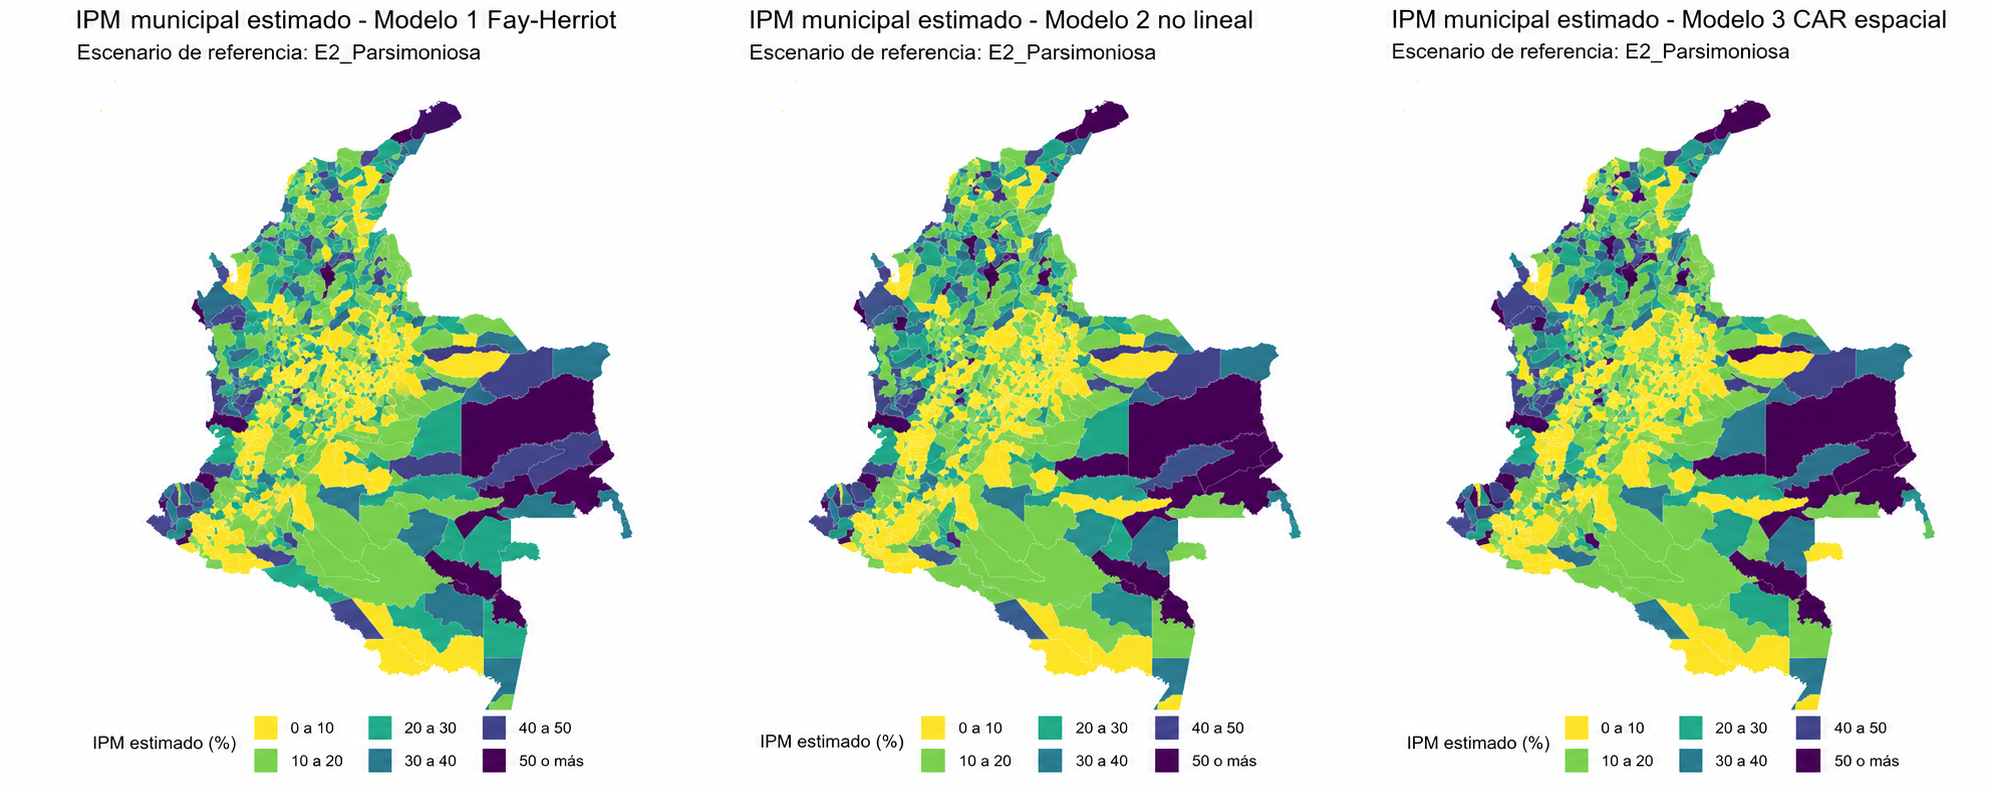
\includegraphics[width=0.95\textwidth]{fig/figures/Panel_Horizontal_Mapas_M1_M2_M3.png}
\caption{Estimación municipal del IPM 2024 bajo el modelo de Fay-Herriot, escenario Parsimonioso.}
\label{fig:Comparacion_Mapas}
\end{figure}

La cartografía permite examinar la distribución territorial generada por cada formulación y complementar las medidas numéricas de concordancia. La proximidad observada entre M2 y M3 en la Tabla~\ref{tab:concordancia-e2} es consistente con la similitud general de sus patrones territoriales, aunque el componente espacial de M3 introduce modificaciones locales asociadas a la estructura de vecindad.

En todos los casos, los mapas tienen una función descriptiva y comparativa. No constituyen una validación independiente de las estimaciones municipales, dado que no se dispone de un IPM municipal directo para 2024 contra el cual contrastarlas.

La comparación visual permitió identificar que las tres formulaciones conservan patrones territoriales generales similares, aunque difieren en la magnitud y en la variación local de las estimaciones. Las diferencias son más evidentes al contrastar la proyección sintética de M1 con las formulaciones M2
y M3, mientras que estas dos últimas presentan una distribución espacial considerablemente más próxima, resultado consistente con las medidas de concordancia municipal.

La incorporación del componente CAR en M3 no produjo una reorganización completa del patrón territorial generado por M2, sino ajustes locales sobre una estructura municipal previamente similar. Estas diferencias cartográficas deben interpretarse conjuntamente con las métricas LODO y las medidas de
concordancia, y no como evidencia independiente de mayor precisión.

En conjunto, la comparación evidencia que los modelos presentan compromisos diferentes entre estabilidad, capacidad predictiva y propiedades estructurales. M1 mostró la mayor estabilidad frente a los escenarios, pero su proyección municipal no garantiza el soporte del indicador. M2 garantizó acotamiento y coherencia departamental y presentó su menor error bajo el escenario Completo. M3 incorporó explícitamente dependencia espacial y alcanzó su menor error bajo el escenario Parsimonioso, aunque fue también la formulación más sensible a los cambios en las covariables. La valoración conjunta de estas dimensiones proporciona la base para la síntesis integrada de validación presentada en la sección siguiente.